\part{Technical description}
\chapter{Hardware}
\section{Introduction to CSAD}
The CS Arctic Drillship was built and instrumented in 2016, with the intention of facilitating more research on Thruster-Assisted Position Mooring. For an in-depth description of the design and construction process, the reader is referred to \cite{bjorno2016thruster}. 

The vessel is a 1:90 scale model of the Statoil Cat I Arctic Drillship. It is equipped with 6 azimuth thruster (3 fore and 3 aft), in addition to a moon-pool for turret and mooring lines. The main dimensions of the vessel are:
\begin{table}[h!]
	\caption{Main dimensions of CSE1}
	\centering
	\begin{tabular}{cc}
		\hline
		LOA & 2.578[m]\\
		B & 0.440 [m]\\
		D & 0.211[m]\\
		T & 0.133[m]\\
		$\Delta$ & 127.92 [kg]\footnote{The weight displacement is based on design loading condition(design water line)}\\\hline
	\end{tabular}
\end{table}

\subsection{Literature}
The development of CSAD and its systems is a product of research from several theses, which contain complementary information on the theory applied to the system. The vessel has also been used in experiments for papers. 
\subsubsection{Journals and conferences}
\begin{itemize}
	\item Modeling, parameter identification and thruster-assisted position mooring of C/S Inoceacn CAT I Drillship \citep{bjorno2017}
	\item Distributed motion sensing on ships \citep{heyn2017}
\end{itemize}
\subsubsection{Specialization projects and master theses}
\begin{itemize}
	\item Thruster-Assisted Position Mooring of C/S Inocean Cat I Drillship \citep{bjorno2016thruster}
	\item Constrained Optimal Thrust Allocation for C/S Inocean Cat I Drillship \citep{frederich2016constrained}
	\item Force Field Identification and Positioning Control of an Autonomous Vessel using Inertial Measurement Units \citep{udjus2017}
	\item Autonomous Heading Control in Position Mooring with Thrust Assist \citep{johannessen2017}
\end{itemize}

\section{Actuators}
The installed azimuth thrusters are of the type Aero-naut Precision Schottel, with 30 millimeter diameter propellers. They are positioned according to the design of the full-scale ship, as given in Figure \ref{fig:thruster_positions} and Table \ref{tab:thruster_positions}. 
\begin{figure}[htb!]
	\centering
	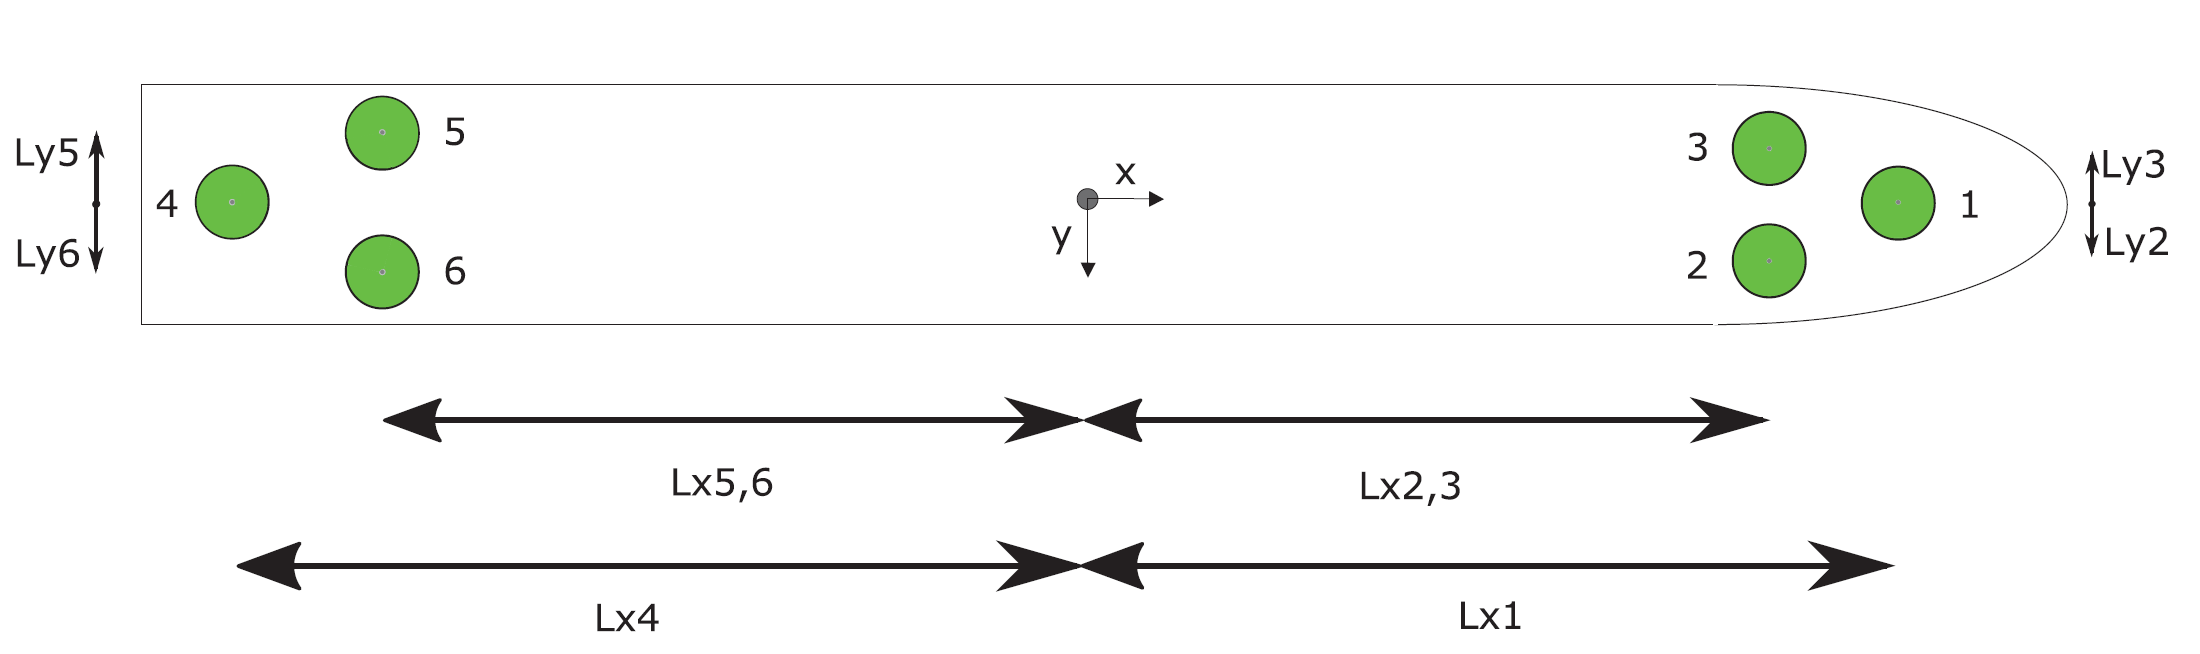
\includegraphics[width=\linewidth]{fig/thruster_position.png}
	\caption{Illustration of thruster positions. Adapted from \cite{frederich2016constrained}}
	\label{fig:thruster_positions}
\end{figure}
\begin{table}[htb!]
	\centering
	\caption{Thruster positions}
	\label{tab:thruster_positions}
	\begin{tabular}{ccc}
		\hline
		\textbf{Thruster} & \textbf{Position X}[m] & \textbf{Position Y}[m]\\ \hline
		Thruster 1 & 1.0678 & 0.0\\
		Thruster 2 & 0.9344 & 0.11\\
		Thruster 3 & 0.9344 & -0.11\\
		Thruster 4 & -1.1644 & 0.0\\
		Thruster 5 & -0.9911 & -0.1644\\
		Thruster 6 & -0.9911 & 0.1644\\ \hline
	\end{tabular}
\end{table}

In \cite{frederich2016constrained}, the thrust coefficients were estimated based on bollard pull tests. The values given in Table \ref{tab:thruster_coefficients} are mean values from the tests, due to discrepancies in the bollard pull test at low thrust commands. 
\begin{table}[htb!]
	\centering
	\caption{Thruster coefficients}
	\label{tab:thruster_coefficients}
	\begin{tabular}{ccccccc}
		\hline
		 & \textbf{Thruster 1} & \textbf{Thruster 2} & \textbf{Thruster 3} & \textbf{Thruster 4} & \textbf{Thruster 5} & \textbf{Thruster 6}\\ \hline
		$K_T$ & 0.3763 & 0.3901 & 0.3776 & 0.5641 & 0.4799 & 0.5588\\
		$K_Q$ & 0.0113 & 0.0117 & 0.0113 & 0.0169 & 0.0144 & 0.0168\\ \hline
	\end{tabular}
\end{table}

\section{Power system}
The vessel is powered through six 12V 12Ah batteries, connected in parallel. Figure \ref{fig:power_system} show a schematic drawing of the power system.

\begin{figure}[h!]
	\centering
	\begin{subfigure}{0.3\textwidth}
		\centering
		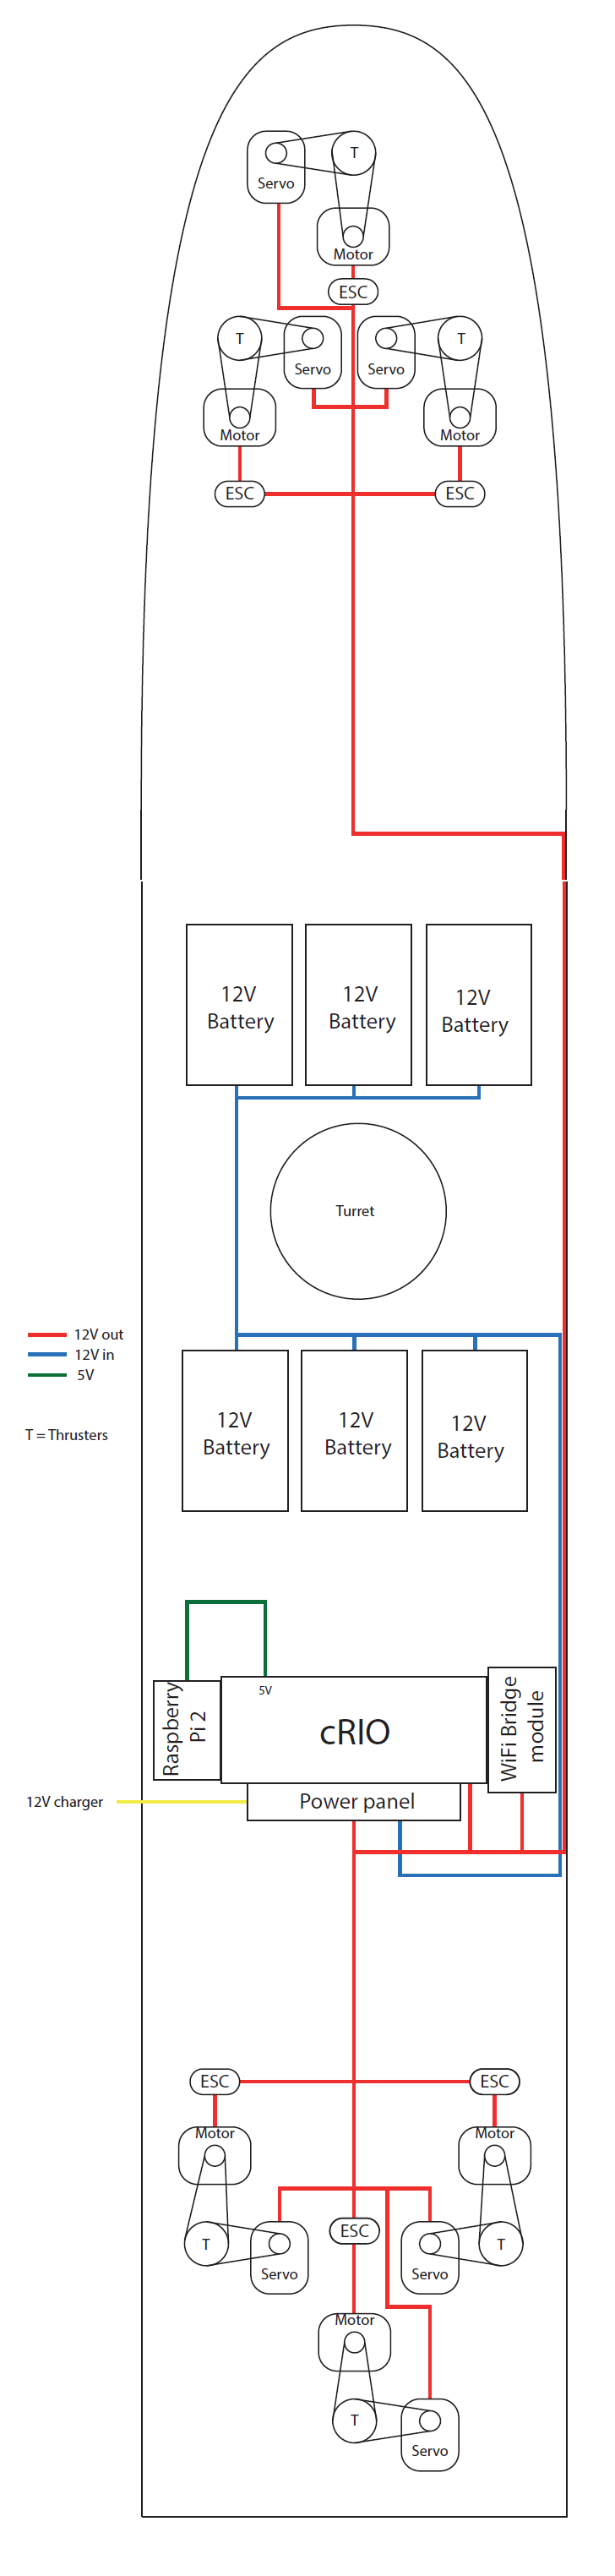
\includegraphics[height=0.9\textheight]{fig/power_system.png}
		\caption{Power system}
		\label{fig:power_system}
	\end{subfigure}
\qquad \qquad
	\begin{subfigure}{0.3\textwidth}
		\centering
		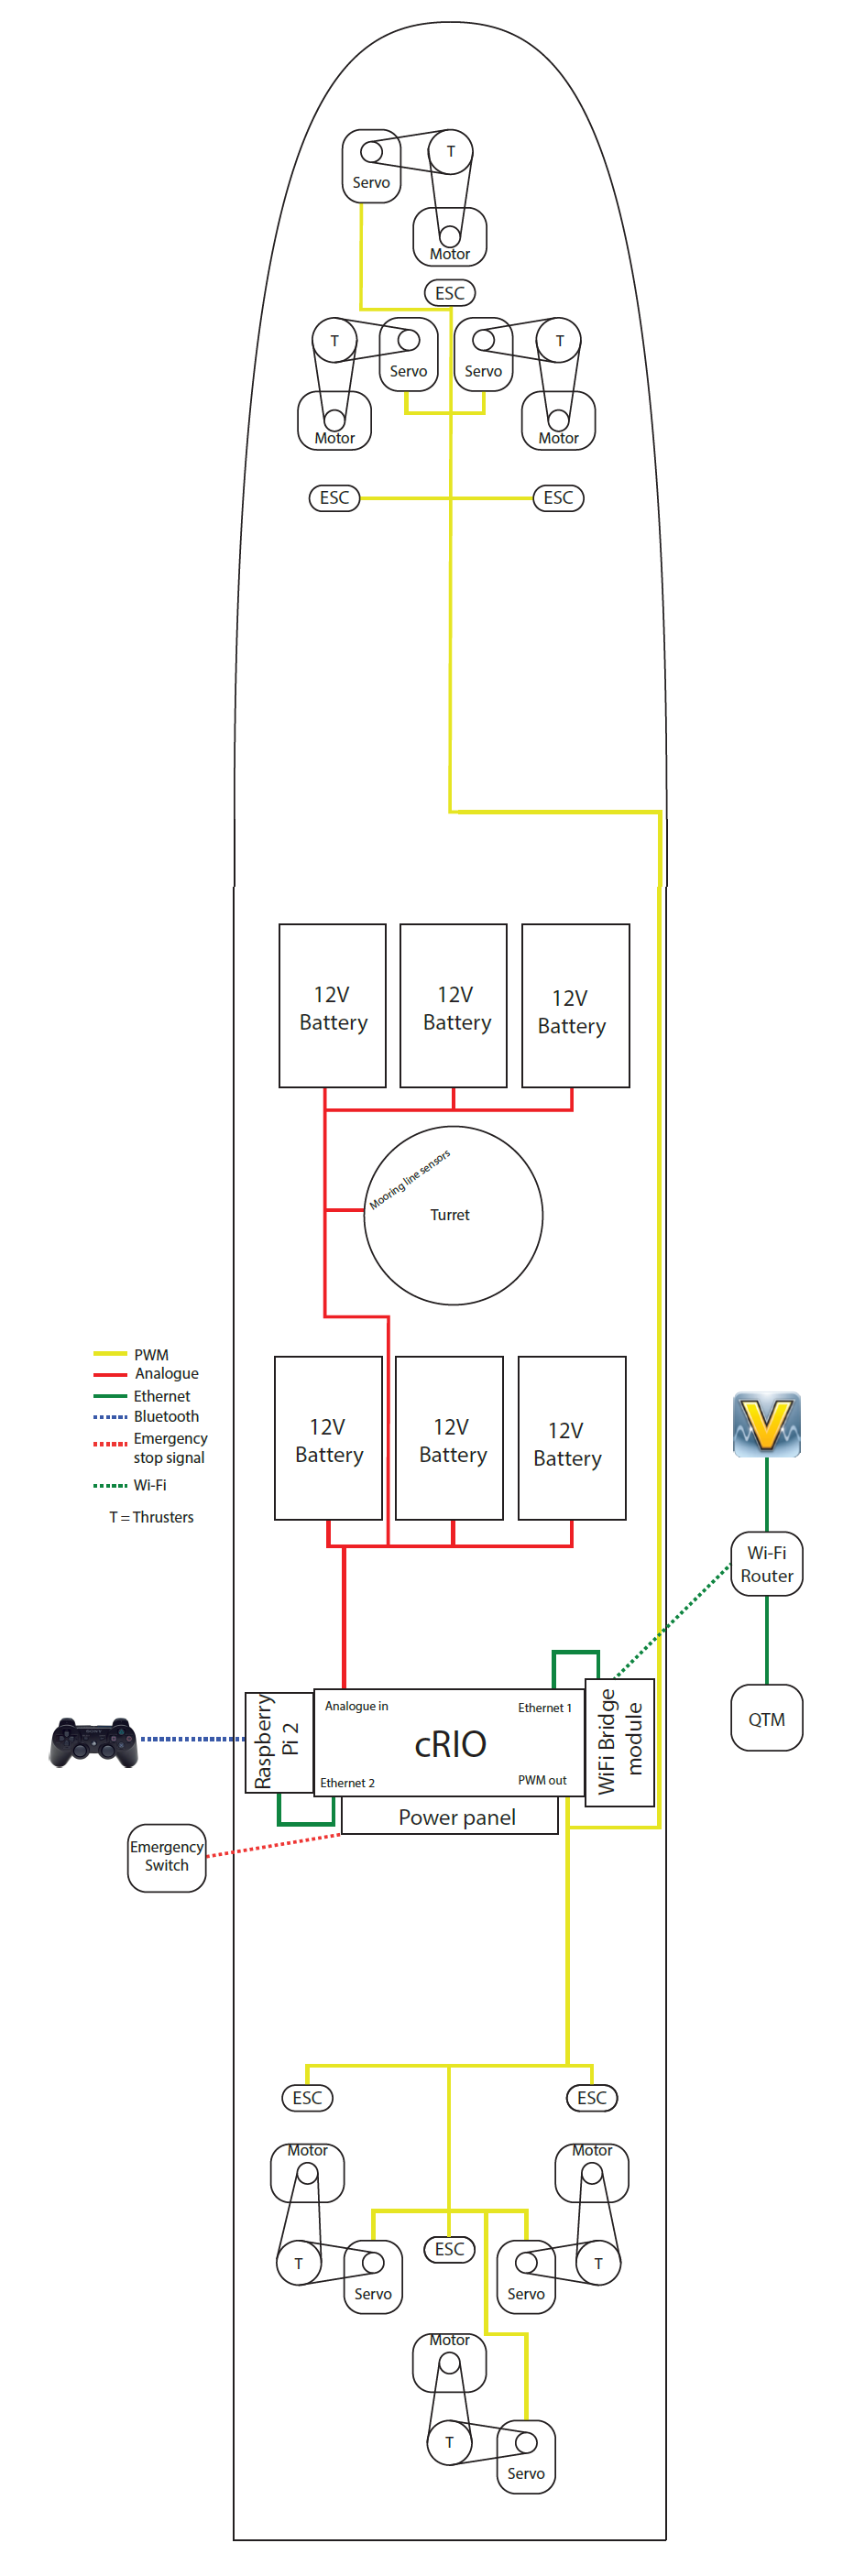
\includegraphics[height=0.9\textheight]{fig/control_system.png}
		\caption{Control system}
		\label{fig:control_system}
	\end{subfigure}
\caption{Illustration of power and control system. Figures adapted from \cite{bjorno2016thruster}.}
\label{fig:power_and_control_system}
\end{figure}
\section{IMU}
CSAD is equipped with one Inertial Measurement Unit (IMU) from Analog Devices. The sensor mounted on-board is the ADIS16364 and includes a triaxis gyroscope and triaxis accelerometer. The sensor has built-in compensation for bias, alignment and sensitivity, and provides accurate measurements over a temperature range of -10 to +70 degrees Celsius. The most relevant data is presented in Table \ref{tab:IMU_specifications}, and for supplementary information the reader is referred to the data sheet \cite{adis16364}. The reference frame of the sensor is illustrated in Figure \ref{fig:IMU_reference_frame}, with positive directions illustrated by arrows. As seen, the standard reference frame for linear accelerations uses left-hand orientation, while the angular rates uses right-hand orientation. It is advised to change the reference frame of accelerations to right-hand, which is achieved by multiplying the accelerations with -1. Note that this also changes the positive direction, defined as the direction of acceleration that produces a positive output. 
\begin{table}[htb!]\caption{IMU specifications}\label{tab:IMU_specifications}
	\centering
	\begin{tabular}{c|c|c|c|}
		\cline{2-4}
		& \textbf{Parameter} & \textbf{Typical value} & \textbf{Unit}\\ \cline{1-4}
		\multicolumn{1}{|c|}{\multirow{5}{*}{\textbf{Gyroscopes}}} & Dynamic range & $\pm 350$ & $^{o}$/sec\\ 
		\multicolumn{1}{|c|}{} & Sensitivity & 0.0125 & $^{o}$/sec/LSB\\ 
		\multicolumn{1}{|c|}{} & Bias stability, $\sigma$ & 0.007 & $^{o}$/sec\\ 
		\multicolumn{1}{|c|}{} & Angular random walk & 2.0 & $^{o}$/$\sqrt{hr}$\\ 
		\multicolumn{1}{|c|}{} & Output noise & 0.8 & $^{o}$/sec rms\\ \cline{1-4}
		
		\multicolumn{1}{|c|}{\multirow{5}{*}{\textbf{Accelerometers}}} & Dynamic range & $\pm 5.25$ & g\\ 
		\multicolumn{1}{|c|}{} & Sensitivity & 1.00 & mg/LSB\\ 
		\multicolumn{1}{|c|}{} & Bias stability, $\sigma$ & 0.1 & mg\\ 
		\multicolumn{1}{|c|}{} & Velocity random walk & 0.12 & m/sec/$\sqrt{hr}$\\ 
		\multicolumn{1}{|c|}{} & Output noise & 5 & mg rms\\ \cline{1-4}
		
		\multicolumn{1}{|c|}{\multirow{1}{*}{\textbf{Power supply}}} & Operating voltage& $5.0 \pm 0.25$ & V\\ \cline{1-4}
	\end{tabular}
\end{table}
\begin{figure}[htb!]
	\centering
	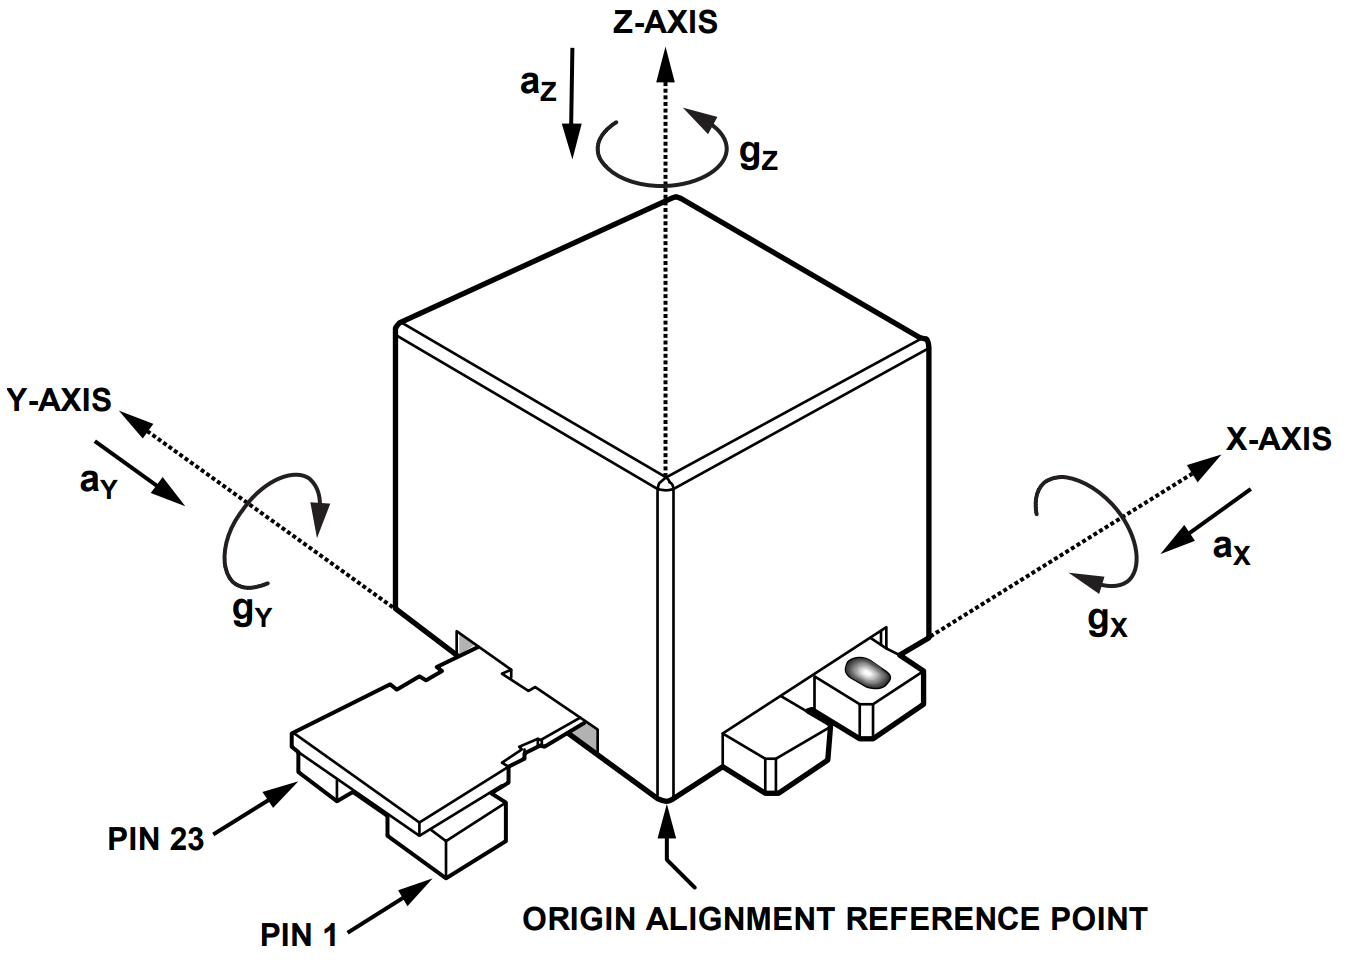
\includegraphics[width=0.6\linewidth]{fig/IMU_reference_frame.png}
	\caption{IMU reference frame from manufacturer}
	\label{fig:IMU_reference_frame}
\end{figure}

\section{Control system}
The on-board control system is illustrated in Figure \ref{fig:control_system}, and consists of the following parts:
\begin{itemize}
	\item one Raspberry pi 4 model b
	\item six electronic speed controllers (ESC) connected to six motors controlling thruster speed
	\item six servos controlling thruster angle
\end{itemize}
For complementary information on the ESC, motors, servos and PWM signals, see \cite{bjorno2016thruster}.
\subsection{RPi}
The Raspberry Pi is running ROS melodic master node at http://192.168.0.123:11311.
Only the ds4\textunderscore driver \textunderscore node is launched at startup to communicate with the ds4 controller. 

\subsection{ESC and DC-motor}
The ESC's are of the type O.S. OCA-150 50 A BL, connected to brushless UMA-2820-950 DC motors driving the thrusters. The ESC's are controlled with PWM signals. As the motors are much more powerful than desired for the model. The servos should not exceed 50\% thrust in either direction.


\subsection{Servo}
The servos controlling the thruster angles are of the type Dynamixel MX-106R, and are geared 1:1 with the thrusters(1 degree turn on servo results in 1 degree on thruster). The servos are manually tuned to have a zero-angle offset in initial start. As of July 2021, the initial offsets are given in Table \ref{tab:angle_offset}.
\begin{equation}\label{eq:maxmin_angle}
	\bm{\alpha} \in [-10240\degree, 10240\degree]
\end{equation}
\begin{table}[htb!]
	\centering
	\caption{Servo angle offset(rad)}
	\begin{tabular}{cc}
		\hline
		\textbf{Thruster} & \textbf{Offset}\\ \hline
		$\alpha_1$ & -0.52\\
		$\alpha_2$ & 1.475\\
		$\alpha_3$ & -1.568\\
		$\alpha_4$ & -1.319\\
		$\alpha_5$ & -0.02\\
		$\alpha_6$ & -1.156\\
		\hline
	\end{tabular}
\label{tab:angle_offset}
\end{table}

The offsets can be changed in the csad\textunderscore actuator\textunderscore driver in src/scad\textunderscore actuator\textunderscore driver.cpp on line 36 in the servoOffsets variable.

\chapter{ROS}
\section{Introduction}
The CSAD is setup to be controlled either directly through a ROS package or through messages sent to a ROS-node running on the ship.

\section{CSAD\textunderscore actuator\textunderscore driver}
csad\textunderscore actuator\textunderscore driver is a package that includes libraries to control CSAD with a couple of simple methods.
csad\textunderscore actuator\textunderscore driver is dependent on the dynamixel\textunderscore sdk ROS library to work.
This means the dynamixel\textunderscore sdk package must be in the same catkin\textunderscore workspace in order to work.

\subsubsection{mapping}

All variables reading and setting the position of the servos are given in rads with 0rads meaning the thruster is pointing directly forward.
All variables setting and reading the power of the motors are mapped from -1.0 to 1.0, with 1 being 100\% forward and -1.0 being 100\% backwards. As the motors are much more powerful than desired for the model the thrust is halved. This means the 1 is actually just 50\% of the capability of the motors. Note that there is nothing in the code stopping anyone from sending 2 and setting the motor to 100\% power.

\subsection{using CSAD\textunderscore Actuator\textunderscore driver library}

To use this library copy folders: csad\textunderscore actuator\textunderscore driver and  dynamixel\textunderscore sdk into the source folder of a catkin workspace. run catkin\textunderscore make in the workspace to build the packages.

\begin{verbatim}
    catkin_make
\end{verbatim}

\noindent Include csad\textunderscore actuator\textunderscore driver in CMakeList.txt the package that is going to be controlling the ship.

\begin{verbatim}
    find_package(catkin REQUIRED COMPONENTS
    csad_actuator_driver
    )
\end{verbatim}

\noindent Include catkin\textunderscore libraries in CMAKEList.txt normally found on line 148 of a standard ros package CMakeList.txt file.

\begin{verbatim}
    Specify libraries to link a library or executable target against
    target_link_libraries(${PROJECT_NAME}
    ${catkin_LIBRARIES}
    )
\end{verbatim}

\noindent Add csad\textunderscore actuator\textunderscore driver in the package.xml file

\begin{verbatim}
    <depend>csad_actuator_driver</depend>
\end{verbatim}

\noindent To use the library simply declare a ship object.

\begin{verbatim}
    CSAD_Actuator ship;
\end{verbatim}
And call the methods included in the library.


\newpage
\subsubsection{Methods}
All methods can be called from any CSAD\textunderscore Actuator object
\begin{itemize}
  \item float getServoPresentPosition(uint8\textunderscore t servoNumber);
  \begin{itemize}
    \item This return the current servo positions of the servo with the number given in the sevoNumber variable.
  \end{itemize}
  \item void getAllServoPresentPositions(double positions[]);  
  \begin{itemize}
    \item This returns all servo positions in the variable positions where the first element corresponds to the servo with the ids specified in the first element of the servoIds variable in csad\textunderscore actuator.cpp
  \end{itemize}
  \item void setServoPosition(double position, uint8\textunderscore t servoNumber);  
  \begin{itemize}
    \item This sets the goal-position of the servo specified in the servoNumber variable, to the position specified in the position variable.
  \end{itemize}
  \item void setAllServoPositions(double positions[NUMBER\textunderscore OF\textunderscore SERVOS]);  
  \begin{itemize}
    \item This sets the goal-positions of all servos to the positions specified in the positions variable, where the first element of the positions array corresponds to the goal-positions of the servo with the id matching the first element of the servosIds array in scad\textunderscore actuator.cpp
    \item The number of elements in position needs to be 6.
  \end{itemize}
  \item void setMotorPower(uint8\textunderscore t motor, double power);  \begin{itemize}
    \item This function sets the motor power of the motor specified in the motor variable, tp the value set in the power variable. 1.0 being 100% forward, and -1.0 being 100% in reverse.
  \end{itemize}
  \item void setAllMotorPower(double power[NUMBER\textunderscore OF\textunderscore SERVOS]);  
  \begin{itemize}
    \item Sets the power of all motors the the values specified in the Power array variable,  1.0 being 100\% forward, and -1.0 being 100\% in reverse.
  \end{itemize}
  \newpage
  \item void closeI2CPort();  
  \begin{itemize}
    \item This closes the I2C port in the raspberry pi, and stops communication with the PCA9685 PWM-module.
  \end{itemize}
  \item void resetPCAModule();  
  \begin{itemize}
    \item Resets the PCA9685 PWM-module.
  \end{itemize}
\end{itemize}

\subsection{controlling CSAD through nodes}
In order to control CSAD through nodes we have to run CSAD\textunderscore node
\begin{verbatim}
    rosrun csad_node CSAD_node
\end{verbatim}
Then we can controll the servos and motors by publishing a std\textunderscore msgs::Float64MultiArray to topic:"CSAD/u". The first six elements corresponds to Thruster power (1 being 100\% and -1 being reverse 100\%) and the last 6 elements corresponds to the angle of the thrusters( -pi being -180deg and pi being 180deg)


\chapter{Modeling}
\section{3 DOF Maneuvering model}
Here, a 3DOF model of the vessel is presented. For complementary information on the procedure and accuracy, the reader is referred to \cite{bjorno2016thruster}. The 3DOF model is based on system identification from towing tests in MC-Lab. The model is valid for low speed, and it is noteworthy that the presented model does not include cross-coupled damping terms. The model is based on the standard 3DOF maneuvering model from \cite{fossen2011handbook}: 
\begin{align}
	\bm{\dot{\eta}}&=\textbf{R}(\psi)\bm{\nu}\\
	\textbf{M}\bm{\dot{\nu}+\textbf{C}(\bm{\nu})\bm{\nu}+\textbf{D}(\bm{\nu})\bm{\nu}}&=\bm{\tau}_{env}+\bm{\tau}_{thruster}
\end{align}
where $\bm{\eta}=[x,y,\psi]^T \in \mathbb{R}^3$, $\bm{\nu}=[u,v,r]^T \in \mathbb{R}^3$ and $\bm{\tau}=[X,Y,N]\in \mathbb{R}^3$. The matrices are
\begin{equation}
	\textbf{R}(\psi)=\left[ \begin{tabular}{ccc}
	$cos(\psi)$ & $-sin(\psi)$ & 0\\
	$sin (\psi)$ & $cos (\psi)$ & 0\\
	0 & 0 & 1
	\end{tabular} \right]
\end{equation}
\begin{equation}
	\textbf{M}=\textbf{M}_{RB}+\textbf{M}_{A}=\left[ \begin{tabular}{ccc}
	$m-X_{\dot{u}}$ & 0 & 0\\
	0 & $m-Y_{\dot{v}}$ & $mx_g-Y_{\dot{r}}$\\
	0 & $mx_g-Y_{\dot{r}}$ & $I_z-N_{\dot{r}}$ 
	\end{tabular} \right] = \textbf{M}^T > 0
\end{equation}
\begin{equation}
	\textbf{C}(\bm{\nu})= \textbf{C}_{RB}(\bm{\nu})+\textbf{C}_A(\bm{\nu})=\left[ \begin{tabular}{ccc}
	0 & $ 0 $ & $(-mx_g+Y_{\dot{r}})r+(-m+Y_{\dot{v}})v$\\
	0 & 0 & $(m-X_{\dot{u}})u$\\
	$(mx_g-Y_{\dot{r}})r+(m-Y_{\dot{v}})v $ & $(-m+X_{\dot{u}})u$ & 0\\
	\end{tabular} \right]
\end{equation}
\begin{equation}
	\textbf{D}(\bm{\nu})=\textbf{D}+\textbf{D}(\bm{\nu})=-\left[\begin{tabular}{ccc}
	$d_{11}(u)$ & 0 & 0\\
	0 & $d_{22}(v)$ & $d_{23}(r)$\\
	0 & $d_{32}(v)$ & $d_{33}(r)$\\
	\end{tabular}
	\right]
\end{equation}
The damping coefficients are 
\begin{align}
	d_{11}(u)&=X_u+X_{|u|u}|u|+X_{uuu}u^2\\
	d_{22}(v,r)&=Y_v+Y_{|v|v}|v|+Y_{vvv}v^2\\
	d_{23}(v,r)&=Y_r+Y_{|r|r}|r|+Y_{rrr}r^2\\
	d_{32}(v,r)&=N_v+N_{|v|v}|v|+N_{vvv}v^2\\
	d_{33}(v,r)&=N_r+N_{|r|r}|r|+N_{rrr}r^2
\end{align}
The rigid body and added mass parameters are given in Table \ref{tab:rigid_body}, and the drag coefficients are given in Table \ref{tab:drag_coeff}. 
\begin{table}[h!]
	\centering
	\caption{Rigid body and added mass parameters}
	\label{tab:rigid_body}
	\begin{tabular}{|cc|c|cc|}
		\cline{1-2}\cline{4-5}
		\multicolumn{2}{|c|}{Rigid body} & \qquad \qquad \qquad & \multicolumn{2}{|c|}{Added mass}\\
		Parameter & Value & & Parameter & Value\\
		\cline{1-2}\cline{4-5}
		$m$ & 127.92 & & $X_{\dot{u}}$ & 3.262\\
		$I_z$ & 61.967 & & $Y_{\dot{v}}$ & 28.89\\
		$x_g$ & 0 & & $Y_{\dot{r}}$ & 0.525\\
		& & & $N_{\dot{v}}$ & 0.157\\
		& & & $N_{\dot{r}}$& 13.98\\
		\cline{1-2}\cline{4-5}
	\end{tabular}
\end{table}
\begin{table}[h!]
	\centering
	\caption{Drag coefficients in surge, sway and yaw}
	\label{tab:drag_coeff}
	\begin{tabular}{|cc|c|cc|c|cc|}
		\cline{1-2}\cline{4-5}\cline{7-8}
		\multicolumn{2}{|c|}{Surge} & \qquad & \multicolumn{2}{|c|}{Sway}& \qquad & \multicolumn{2}{|c|}{Yaw}\\
		Parameter & Value & & Parameter & Value & & Parameter & Value\\
		\cline{1-2}\cline{4-5}\cline{7-8}
		$X_u$ & -2.332 & & $Y_v$ & -4.673 & & $N_r$ & -0.01675\\
		$X_{|u|u}$ & 0 & & $Y_{|v|v}$ & 0.3976 & & $N_{|r|r}$ & -0.01148\\
		$X_{uuu}$ & -8.557 & & $Y_{vvv}$ & 313.3 & & $N_{rrr}$ & 0.0003578\\
		\cline{1-2}\cline{4-5}\cline{7-8}
	\end{tabular}
\end{table}